\documentclass[mathserif]{beamer}
\usepackage[utf8]{inputenc}
\usepackage{amsmath}
\usepackage{amsfonts}
\usepackage{amssymb}
\usepackage{arydshln}
\usepackage{graphicx}
\usepackage{float}
\usepackage{picture}
\usepackage{dcolumn}
\usepackage{textpos}
\usepackage{graphicx}
\usepackage{subcaption}

\setbeamercolor{structure}{fg=grey}
\usetheme[sectionpage=progressbar, progressbar=frametitle]{metropolis}

\definecolor{prettyBlue}{HTML}{2196F3}
\setbeamercolor{progress bar}{fg=prettyBlue, bg=gray}

%Information to be included in the title page:
\title{Development of a Pendulum Control System}
\author{Thomas S. Christensen \\ Mikkel S. Jaedicke\\}

\institute{University of Southern Denmark}
\date{Jan, 2018} 

\addtobeamertemplate{frametitle}{}{%
\begin{textblock*}{200mm}(\textwidth-1.5cm,-0.8cm)

\includegraphics[scale=0.15]{graphics/sdu_logo}
\end{textblock*}}

\begin{document}

\begin{frame}[t]\frametitle{~}
\maketitle
\end{frame}

\begin{frame}[c]\frametitle{Agenda}
\setbeamertemplate{section in toc}[sections numbered]
\tableofcontents[hideallsubsections]
\end{frame}


\section{Introduction}

\begin{frame}[c]\frametitle{System Overview}

\centering
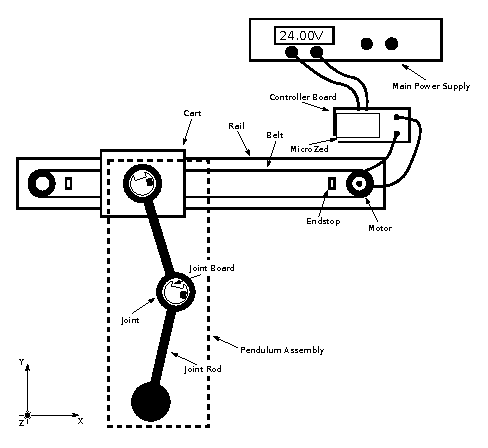
\includegraphics[scale=1]{graphics/system_overview}
\end{frame}

\begin{frame}[c]\frametitle{Implemented System}
\centering
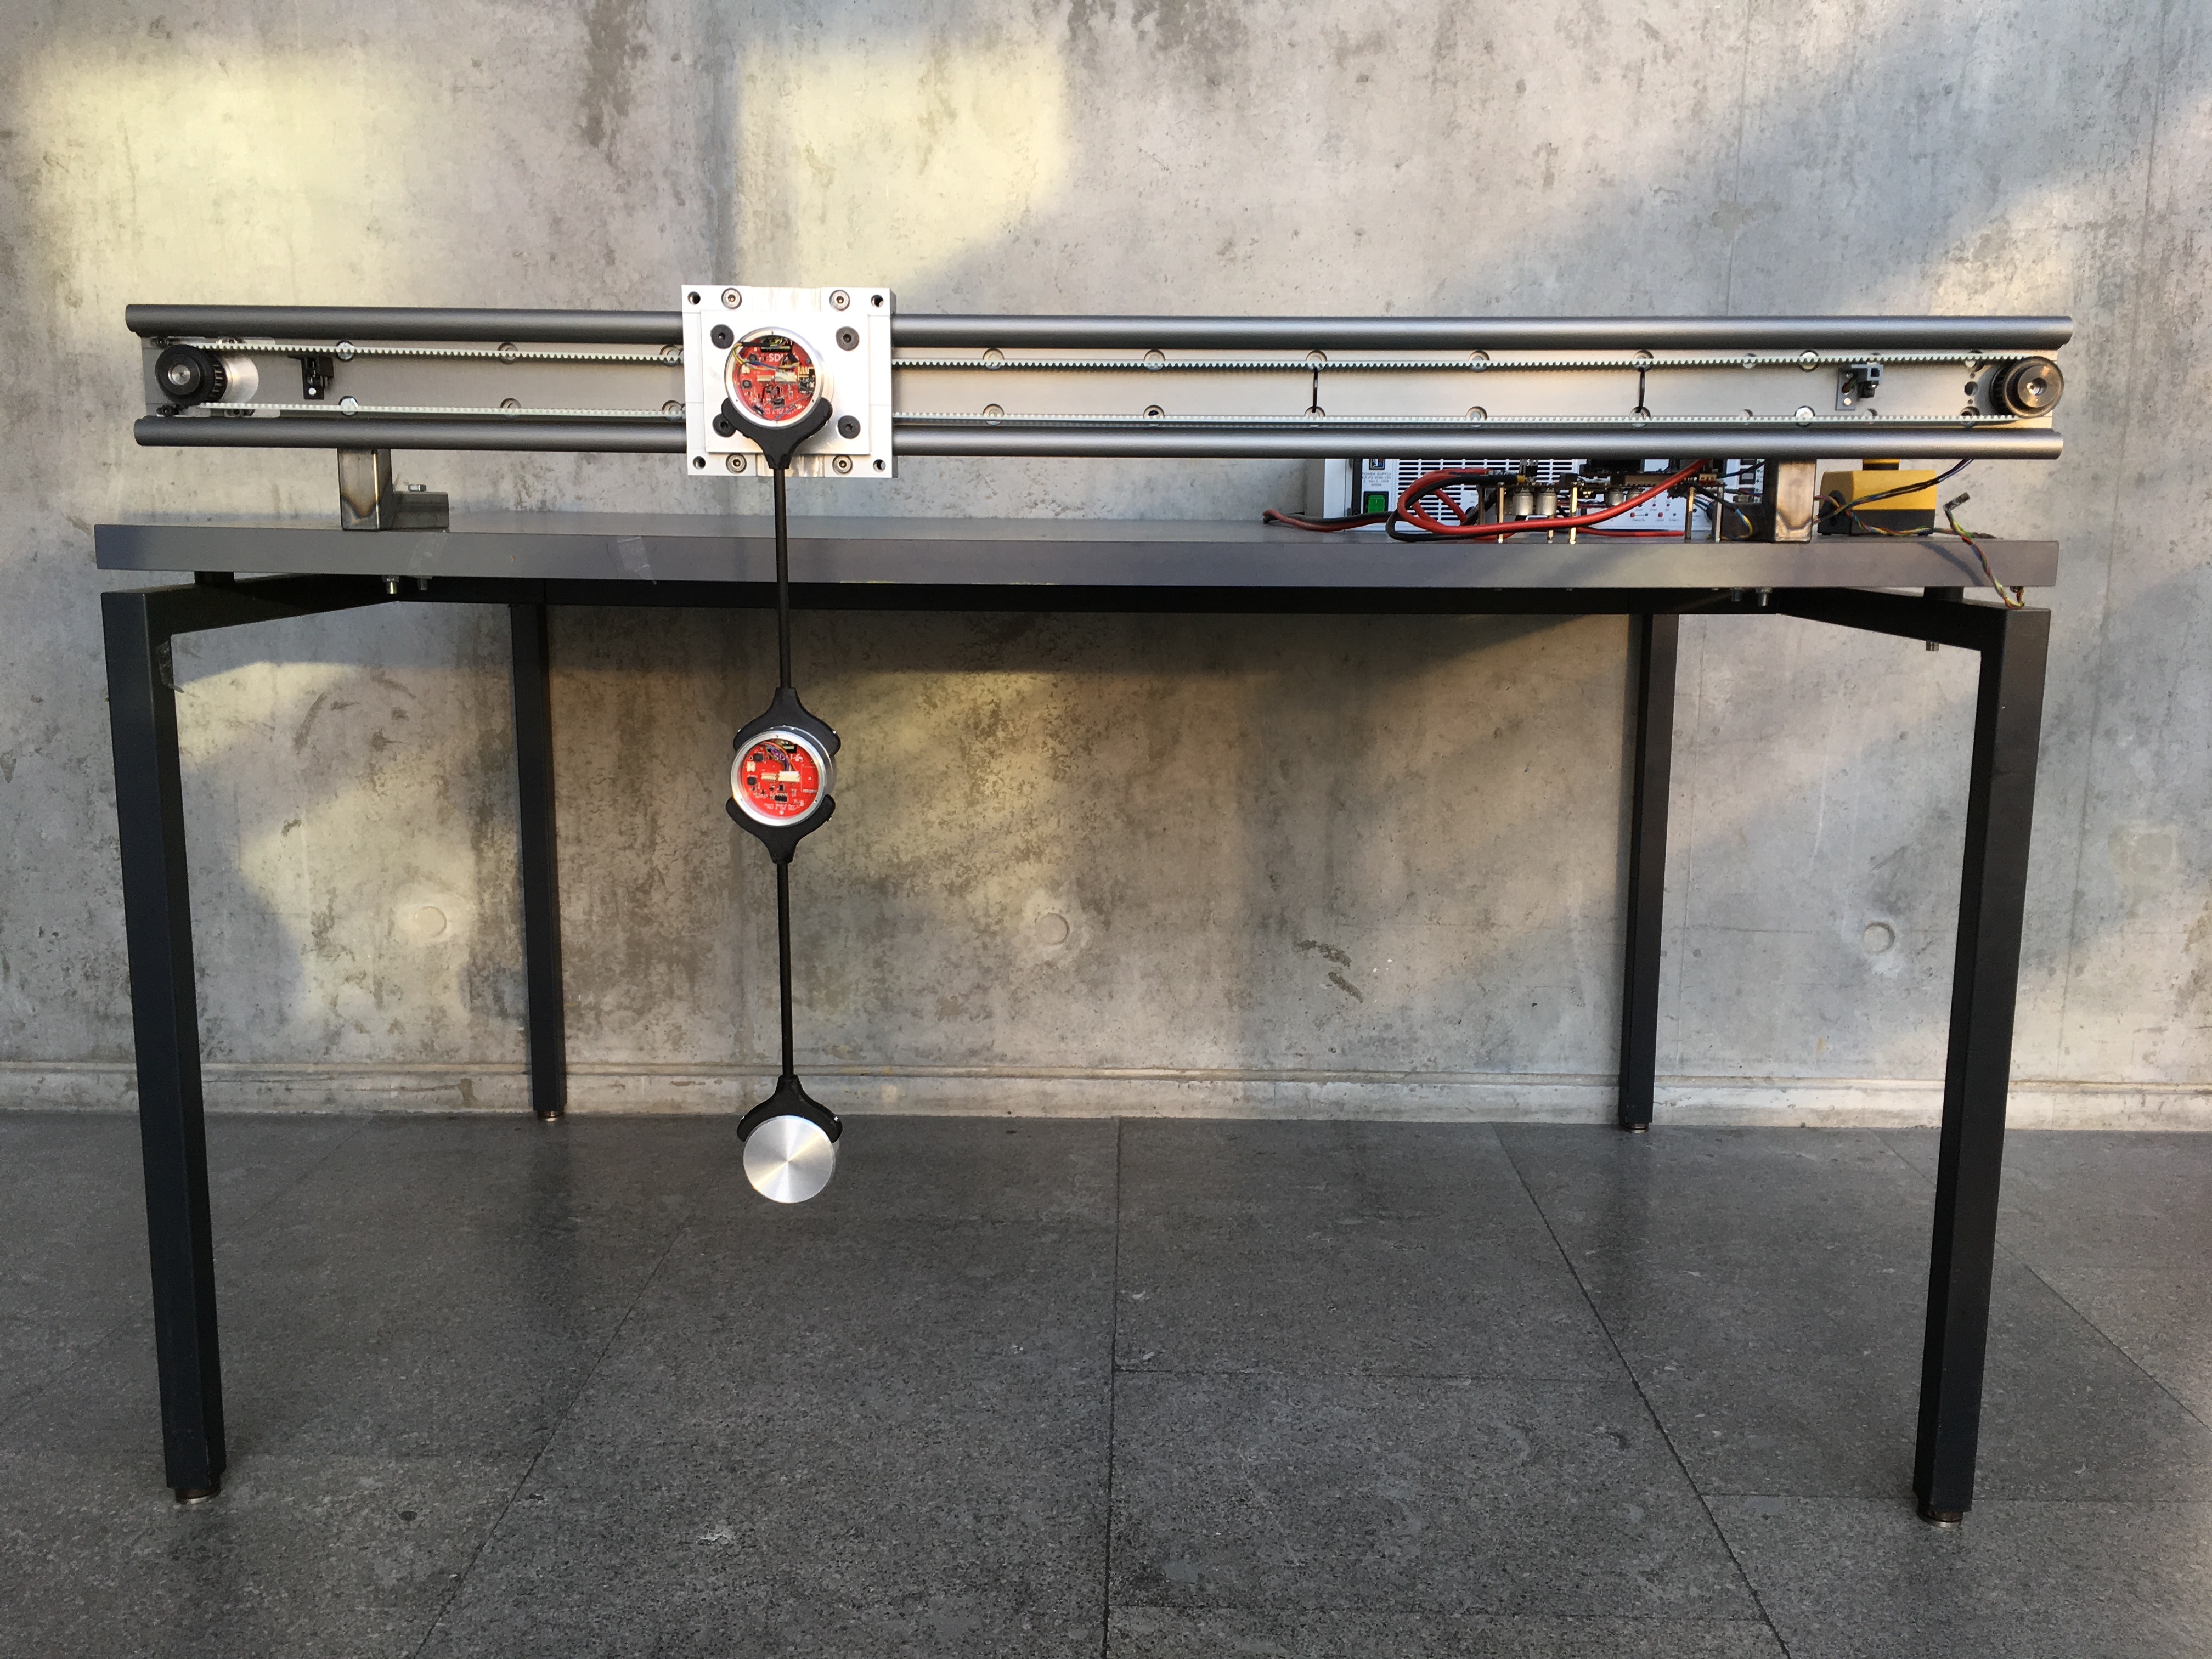
\includegraphics[width=0.9\textwidth]{graphics/full_system_finish}
\end{frame}

\begin{frame}[c]\frametitle{Workflow}
\centering
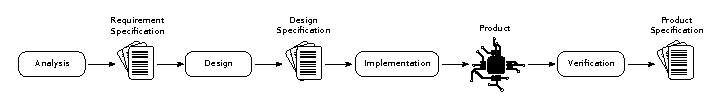
\includegraphics[width=\textwidth]{graphics/workflow}    
\end{frame}


\section{Analysis}

\begin{frame}[t]\frametitle{Analysis}
    Something here?!
\end{frame}

\begin{frame}[c]\frametitle{Requirement Specification}

\textbf{Functional:}
\begin{enumerate}
	\item System should consists of a double pendulum mounted on a moveable cart.
	\item Cart should be actuated by the Maxon 148867. 
	\item The pendulum system should be controlled by a MicroZed.
	\item \alert{Position of the cart and joint angles should be measured.}
\end{enumerate}

\end{frame}

\section{Design}

\begin{frame}{Mechanical Design}
	\begin{figure}
	\centering
	\begin{subfigure}{.5\textwidth}
	  \centering
	  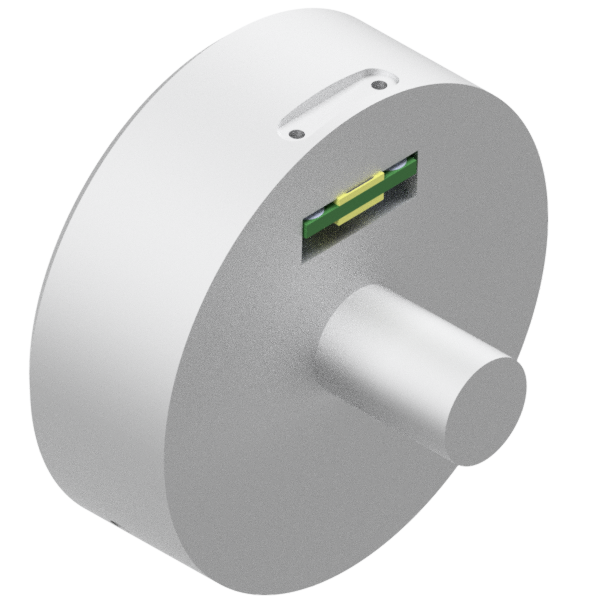
\includegraphics[width=.9\linewidth]{graphics/joint_read_side}
	\end{subfigure}%
	\begin{subfigure}{.5\textwidth}
	  \centering
	  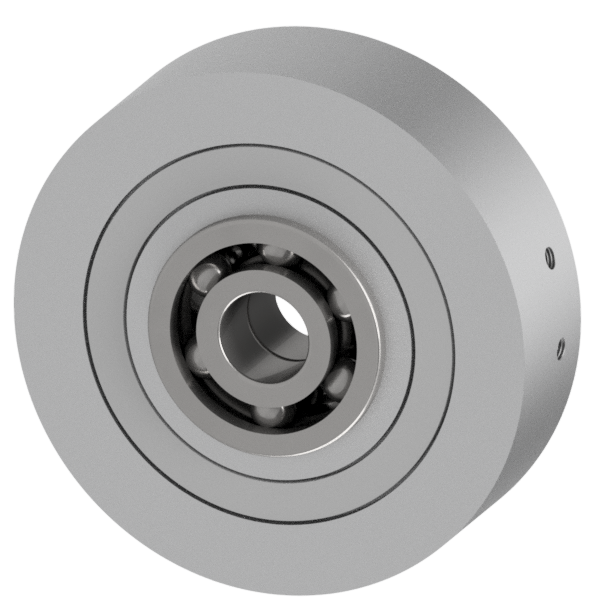
\includegraphics[width=.9\linewidth]{graphics/joint_mag_assembly}
	\end{subfigure}
	\end{figure}
\end{frame}

\begin{frame}[t]\frametitle{Electrical Design}
    
\end{frame}

\begin{frame}{Software Design}
	\begin{figure}
	\centering
	  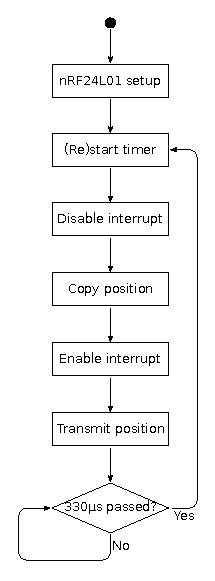
\includegraphics[width=.25\linewidth]{graphics/joint_software_diagram}
	\end{figure}
\end{frame}


%\begin{frame}{Software Design}
%	\begin{figure}
%	\centering
%	  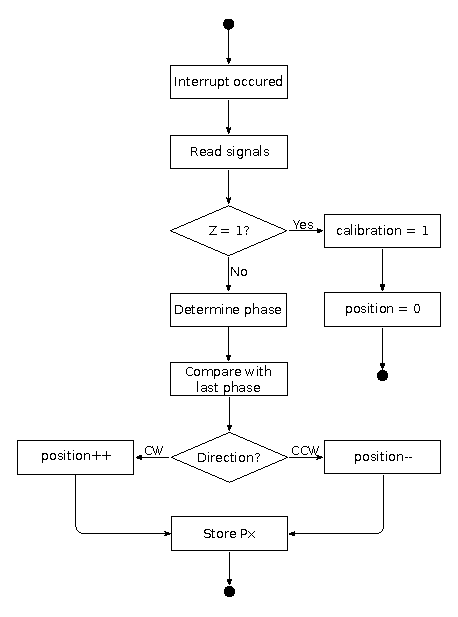
\includegraphics[width=.55\linewidth]{graphics/joint_interrupt}
%	\end{figure}
%\end{frame}



\begin{frame}{First Frame}
Hello, world!
\end{frame}



\begin{frame}[standout]
  Questions?
\end{frame}

\end{document}